\documentclass[11pt]{article}
\usepackage{natbib}
\usepackage{float}
\usepackage[pdftex]{graphicx}     % could insert ``draft'' between []
\usepackage{amsmath}
\pagestyle{empty}
\setlength{\oddsidemargin}{0pt}
\setlength{\textwidth}{6.5in}
\setlength{\voffset}{0pt}
\setlength{\topmargin}{-0.75in}
\setlength{\textheight}{10.0in}
%%%%%%%%%%%

\newcommand{\inch}{$^{\prime\prime}$}
\newcommand{\foot}{$^{\prime}$}
\renewcommand{\deg}{^\circ}

\begin{document}
\title{Diameter of the HERA Antenna}
\author{David DeBoer and Aaron Parsons}
\maketitle

The diameter of the HERA antenna is set by three factors:  (1) meeting the delay reflection specification of 60 dB at 60 ns, (2) lessening the impact of systematics, (3) lessening cost for a fixed sensitivity.

\section{Delay}
The delay-delayrate analysis technique employed for HERA requires that the region of phase space employed has contamination below the level of the signal.  The supplied value from the analysis team is that reflections must be reduced by at least 60 dB at 60 ns.  Another formulation is VSWR $<$ 1.002 at frequencies below 15 MHz.  The reflections between the feed and vertex is a chief contributor.  The determine the delay scale a focal ratio must be used.  A series of analytical models was run at several diameters using the calculated beam pattern of the PAPER feed.  The results are shown in Figure \ref{fig:efficiency}.  Note that they all peak at about a focal ratio of 0.32 (the solid lines with the x-axis divided by 10).

\begin{figure}[h]
\centering
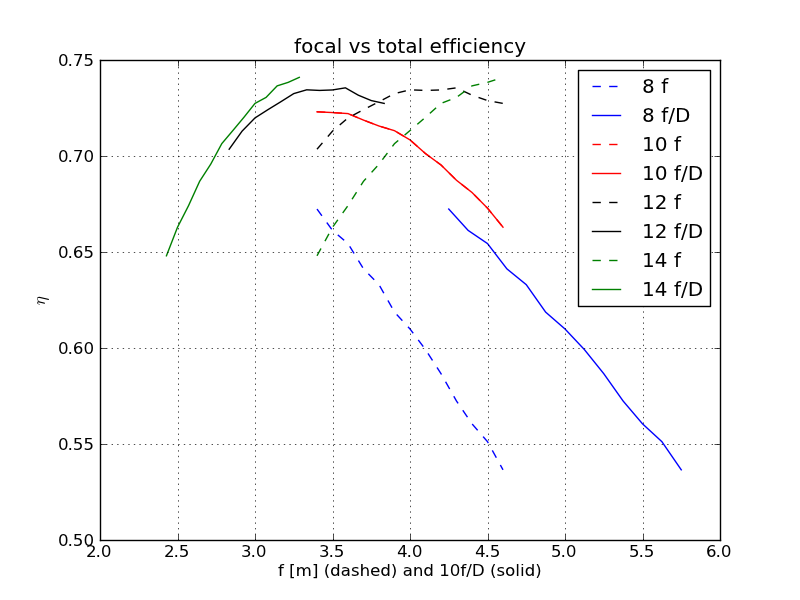
\includegraphics[width=0.8\textwidth]{heraDishfDplot.png}
\caption{Efficiencies of various diameters and focal lengths in one confusing plot.}
\label{fig:efficiency}
\end{figure}

Using an $f/D=0.32$, one can compute the round-trip times between the vertex and feed.  Figure \ref{fig:roundtrip} shows the round-trip ({\em i.e.} delay) times for 1, 2 and 3 trips with a vertical line at 60 ns, the delay spec.  This may be interpreted that for diameters of about 28-m you have one round-trip in which to attenuate by 60 dB, for a diameter of about 14-m  you have two round-trips and for diameters of about 9.4-m you have three round-trips. 
\begin{figure}[h]
\centering
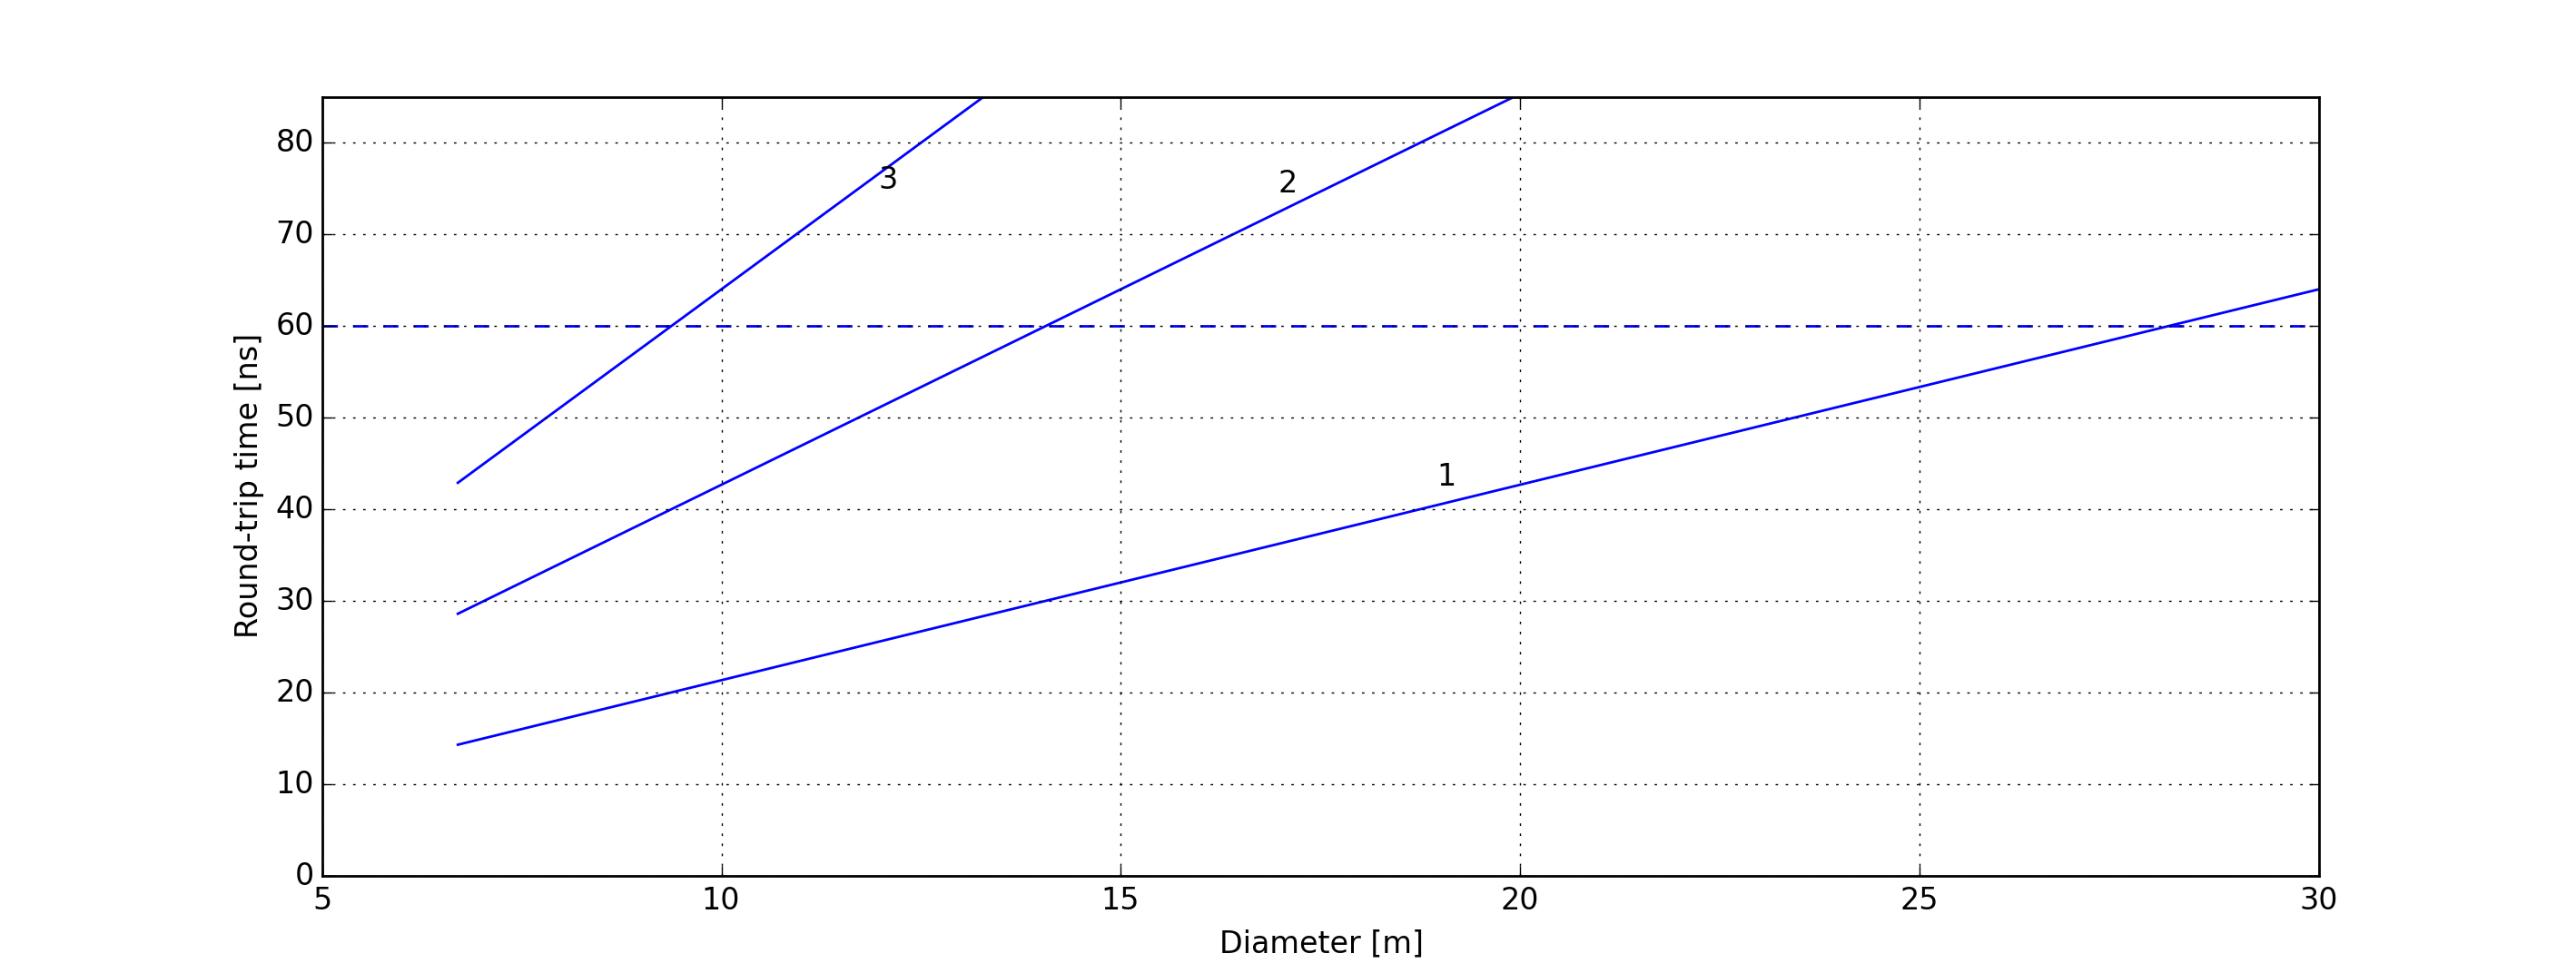
\includegraphics[width=1.0\textwidth]{roundtrip.png}
\caption{Round-trip times for $f/D=0.32$ for 1, 2 and 3 trips.}
\label{fig:roundtrip}
\end{figure}

If we assume an "attenuation/bounce" that takes into account the loss factors at each segment of the round-trip journeys (reflections, path loss, etc -- so we could have partial round-trips) we can look over a plausible range and see if they might feasibly provide enough overall attenuation.  Figure \ref{fig:bounces} plots this for 1, 2 and 3 round-trips.
\begin{figure}[h]
\centering
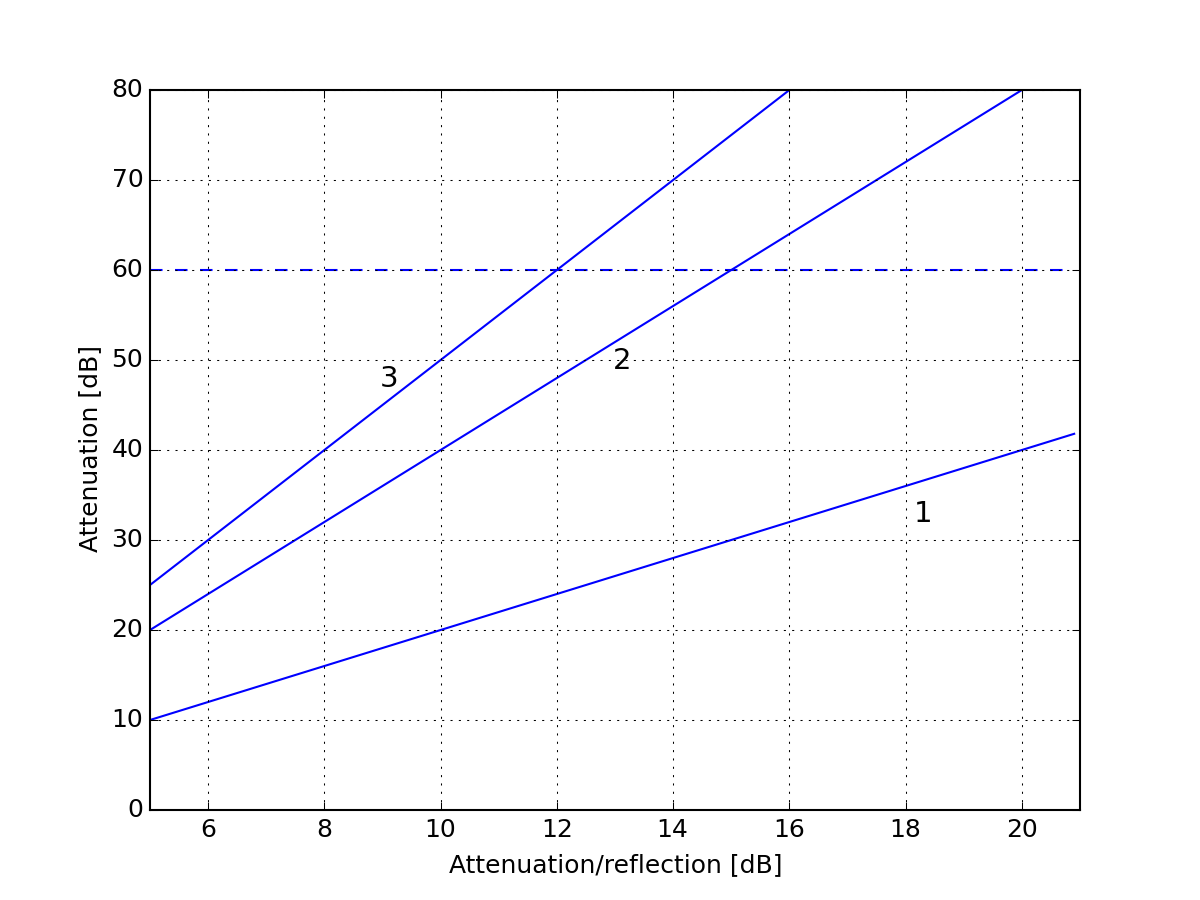
\includegraphics[width=1.0\textwidth]{bounces.png}
\caption{Overall attenuation for 1, 2 and 3 trips.}
\label{fig:bounces}
\end{figure}

One interpretation of the above is that we should have a diameter of 14-m or less and make sure we have 20 dB or more per "bounce".  

INCLUDE PLOT OF RELECTOMETRY TESTS

\section{Systematics}
Fringe rotation, cross-talk

\section{Sensitivity}
The equation for sensitivity has been described in previous works [REFS] and depends on many parameters
related to the instrumentation, the configuration, the location, the observing strategy, etc.  A useful form for 
the proposed compact configuration is Eq 27 in \citep{Parsonsetal2012} and reproduced here:
\begin{equation}
\centering
\label{eq:sensitivity}
\begin{split}
\Delta^2_N(k) \approx 60 \left[\frac{k}{0.1h\text{Mpc}^{-1}}\right]^\frac{5}{2}
                                         \left[\frac{6 \text{MHz}}{B}\right]^\frac{1}{2}
                                         \left[\frac{1}{\Delta\ln k}\right]^\frac{1}{2} \\
                        \times       \left[\frac{\Omega}{0.76\text{sr}}\right]
                                         \left[\frac{T_\text{sys}}{500 \text{K}}\right]^2
                                         \left[\frac{6 \text{hrs}}{t_\text{per\_day}}\right]^\frac{1}{2} \\
                        \times       \left[\frac{120\text{days}}{t_{\text{cam}}}\right]
                                         \left[\frac{32}{N_a}\right]
                                         \left[\frac{\text{10}^4f_o}{f}\right]  \text{mK}^2
\end{split}
\end{equation}
where $k$ is the magnitude of the $k$-mode, $B$ is the bandwidth, $\Delta\ln k$ is the log
of the binsize, $\Omega$ is the field-of-view, $T_{\text{sys}}$ is the system temperature, 
${t_\text{per\_day}}$ is the number of hours observed per day, $t_{\text{cam}}$ is the number of days
observed, $N_a$ is the number of antennas, and $f_o/f$ is the configuration metric for a 
redundant array as defined in \citep{Parsonsetal2012}.

Note that $\Delta^2_N(k)$ is the standard radiometric sensitivity equation, scaled by
the volume in $k$-space, normalized by the power spectrum Fourier coefficient, and
reduced by the number of independent samples in a given $k$-mode bin, which may have
both coherent and incoherent application.

Pulling out terms relating to diameter ($D_a$) and number, we can write Eq. \ref{eq:sensitivity} as
\begin{equation}
\label{eq:reducedSensitivity}
\Delta^2_N(k) \propto \frac{\Omega (f_o/f)}{N_a\sqrt{t_\text{per\_day}}} \propto \frac{(1/D_a^2)(1/\sqrt{N_a})}{N_a\sqrt{D_a}}
= D_a^{-\frac{5}{2}}N_a^{-\frac{3}{2}}
\end{equation}
where the dependencies on diameter and number have been substituted in, noting that the expressions for $f_o/f$ and 
$t_\text{per\_day}$were derived in Parsons et al where the baselines for the close-packed array are multiples of the diameter.

Letting the reduced sensitivity be $C = D_a^{-\frac{5}{2}}N_a^{-\frac{3}{2}}$ and scaling for canonical values of $D_a = 14$ m, $N_a = 331$ m, the needed number of antennas as a function of diameter (shown in Fig \ref{fig:Nsens}) is
\begin{equation}
\label{eq:Nmetric}
N_a = 26918 D_a^{-\frac{5}{3}}
\end{equation}

\begin{figure}[h]
\centering
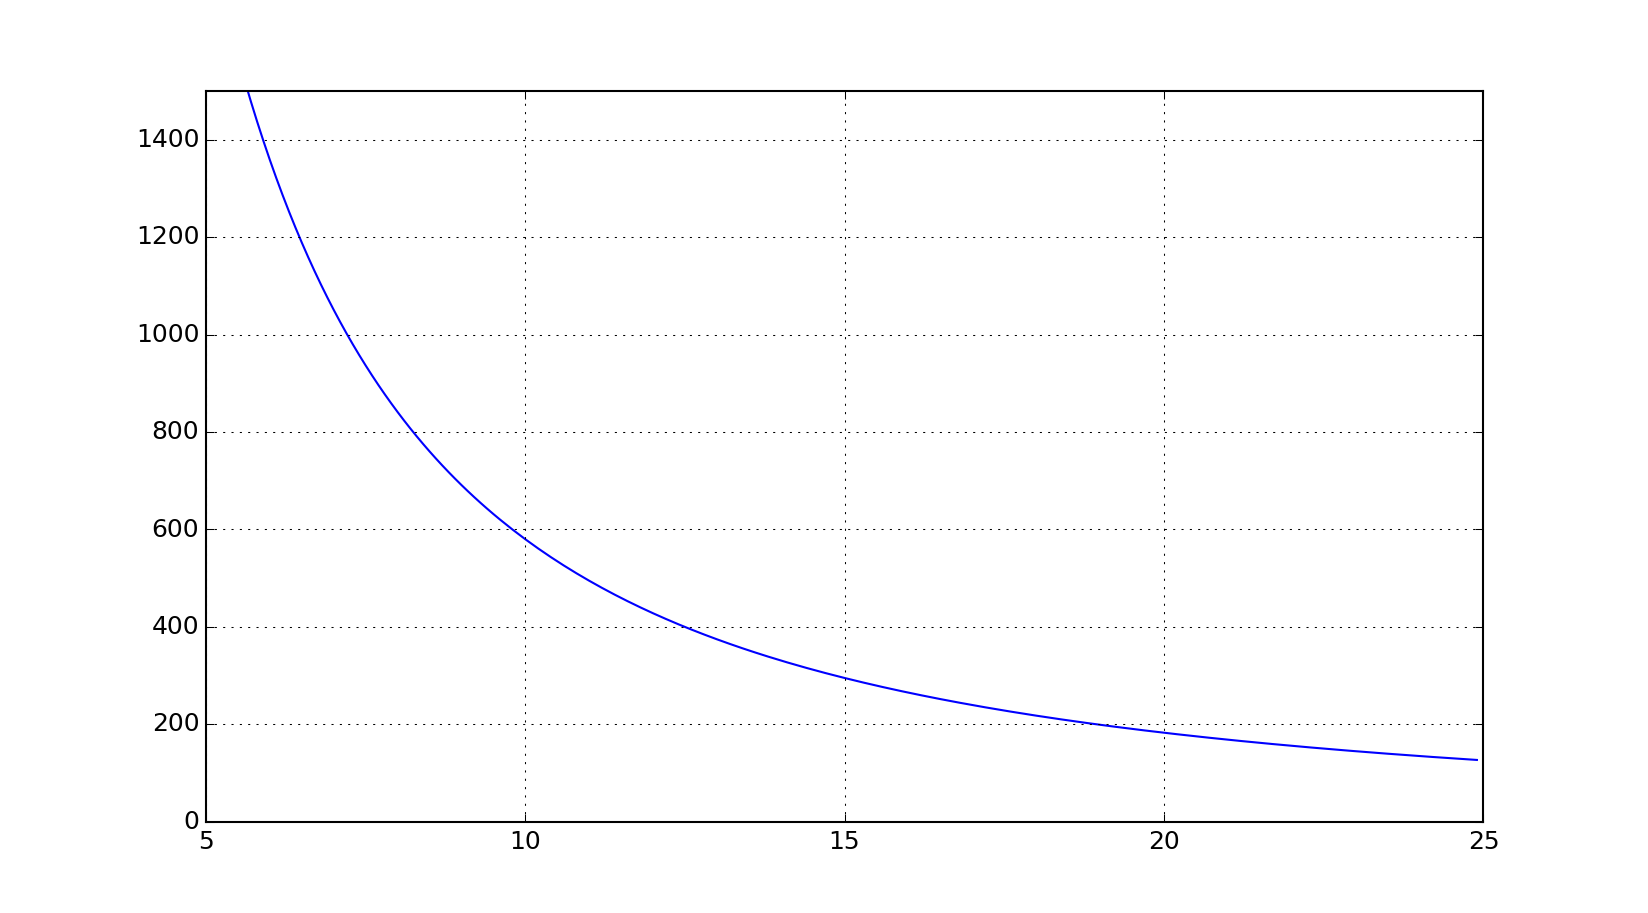
\includegraphics[width=0.8\textwidth]{Nsens.png}
\caption{Number of antennas at fixed sensitivity with reference of 331 14-m antennas}
\label{fig:Nsens}
\end{figure}

The sensitivity specification is to maximize performance per cost, which determines the element 
diameter ($D_a$) and the number of elements ($N_a$) subject to the constraints above.  One therefore 
needs a model of cost and performance as a function of $D_a$ and $N_a$.  Given a fairly mature element
and system design, a bottoms-up costing appropriate for element diameters from about 6-m to 30-m 
has been done for hex-numbers corresponding to element counts from 91 to 1141.  The costs here
are only those associated with delivering the array to that scope on-site, so excluding development and
science.  The results are shown in Fig. \ref{fig:normcost}.  At diameters greater than about 12-m the cost function
is relatively flat.

\begin{figure}[h]
\centering
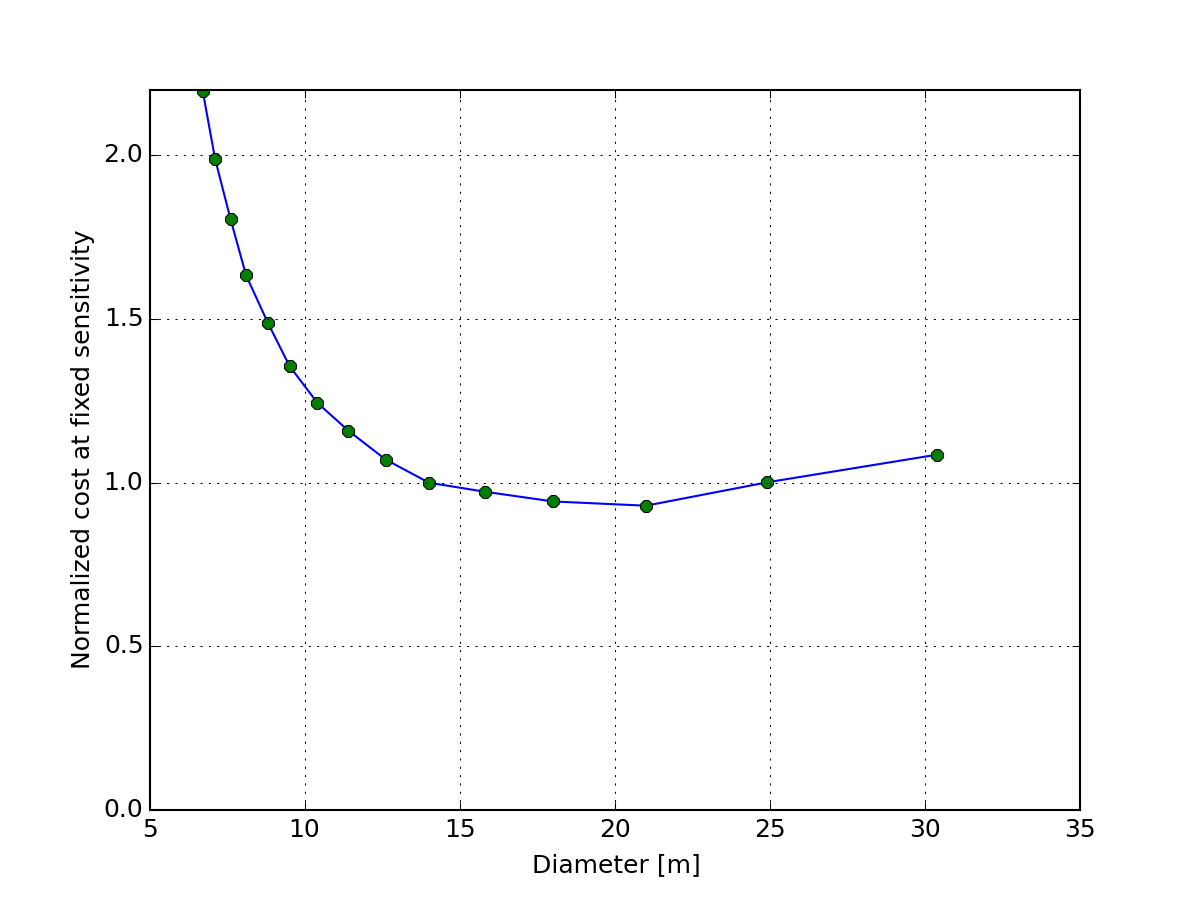
\includegraphics[width=0.8\textwidth]{normcostfunc.png}
\caption{Normalized cost at fixed sensitivity with reference of 331 14-m antennas}
\label{fig:normcost}
\end{figure}

\bibliographystyle{plainnat}
\bibliography{YOUR BIBLIOGRAPHY HERE}
\end{document}